% TODO move to a higher level (working methods?)
% A coding-standard was quickly decided on to make sure the code style was somewhat coherent effectively making it easier for different members to take over other members code if needed.

The backend was developed using JavaScript running with \nodejs{} as server framework and Express as a web framework to handle routing. \nodejs{} was chosen because it was the most established framework with wide support and multiple extensions, such as Express.

\subsection{Database} \label{database}

%OLD TEXT COMMENTED
%The document database MongoDB was chosen for the project instead of using a relational database, %the reasoning for this decision was to have a database that was built with scalability in mind %and dynamic schemas but also because of the simple reason that it is easy for the programmers to %read and understand the data inside the database thanks to MongoDBs JSON-like document %structure.
%OLD TEXT COMMENTED

\begin{sidewaysfigure}
    \centering
    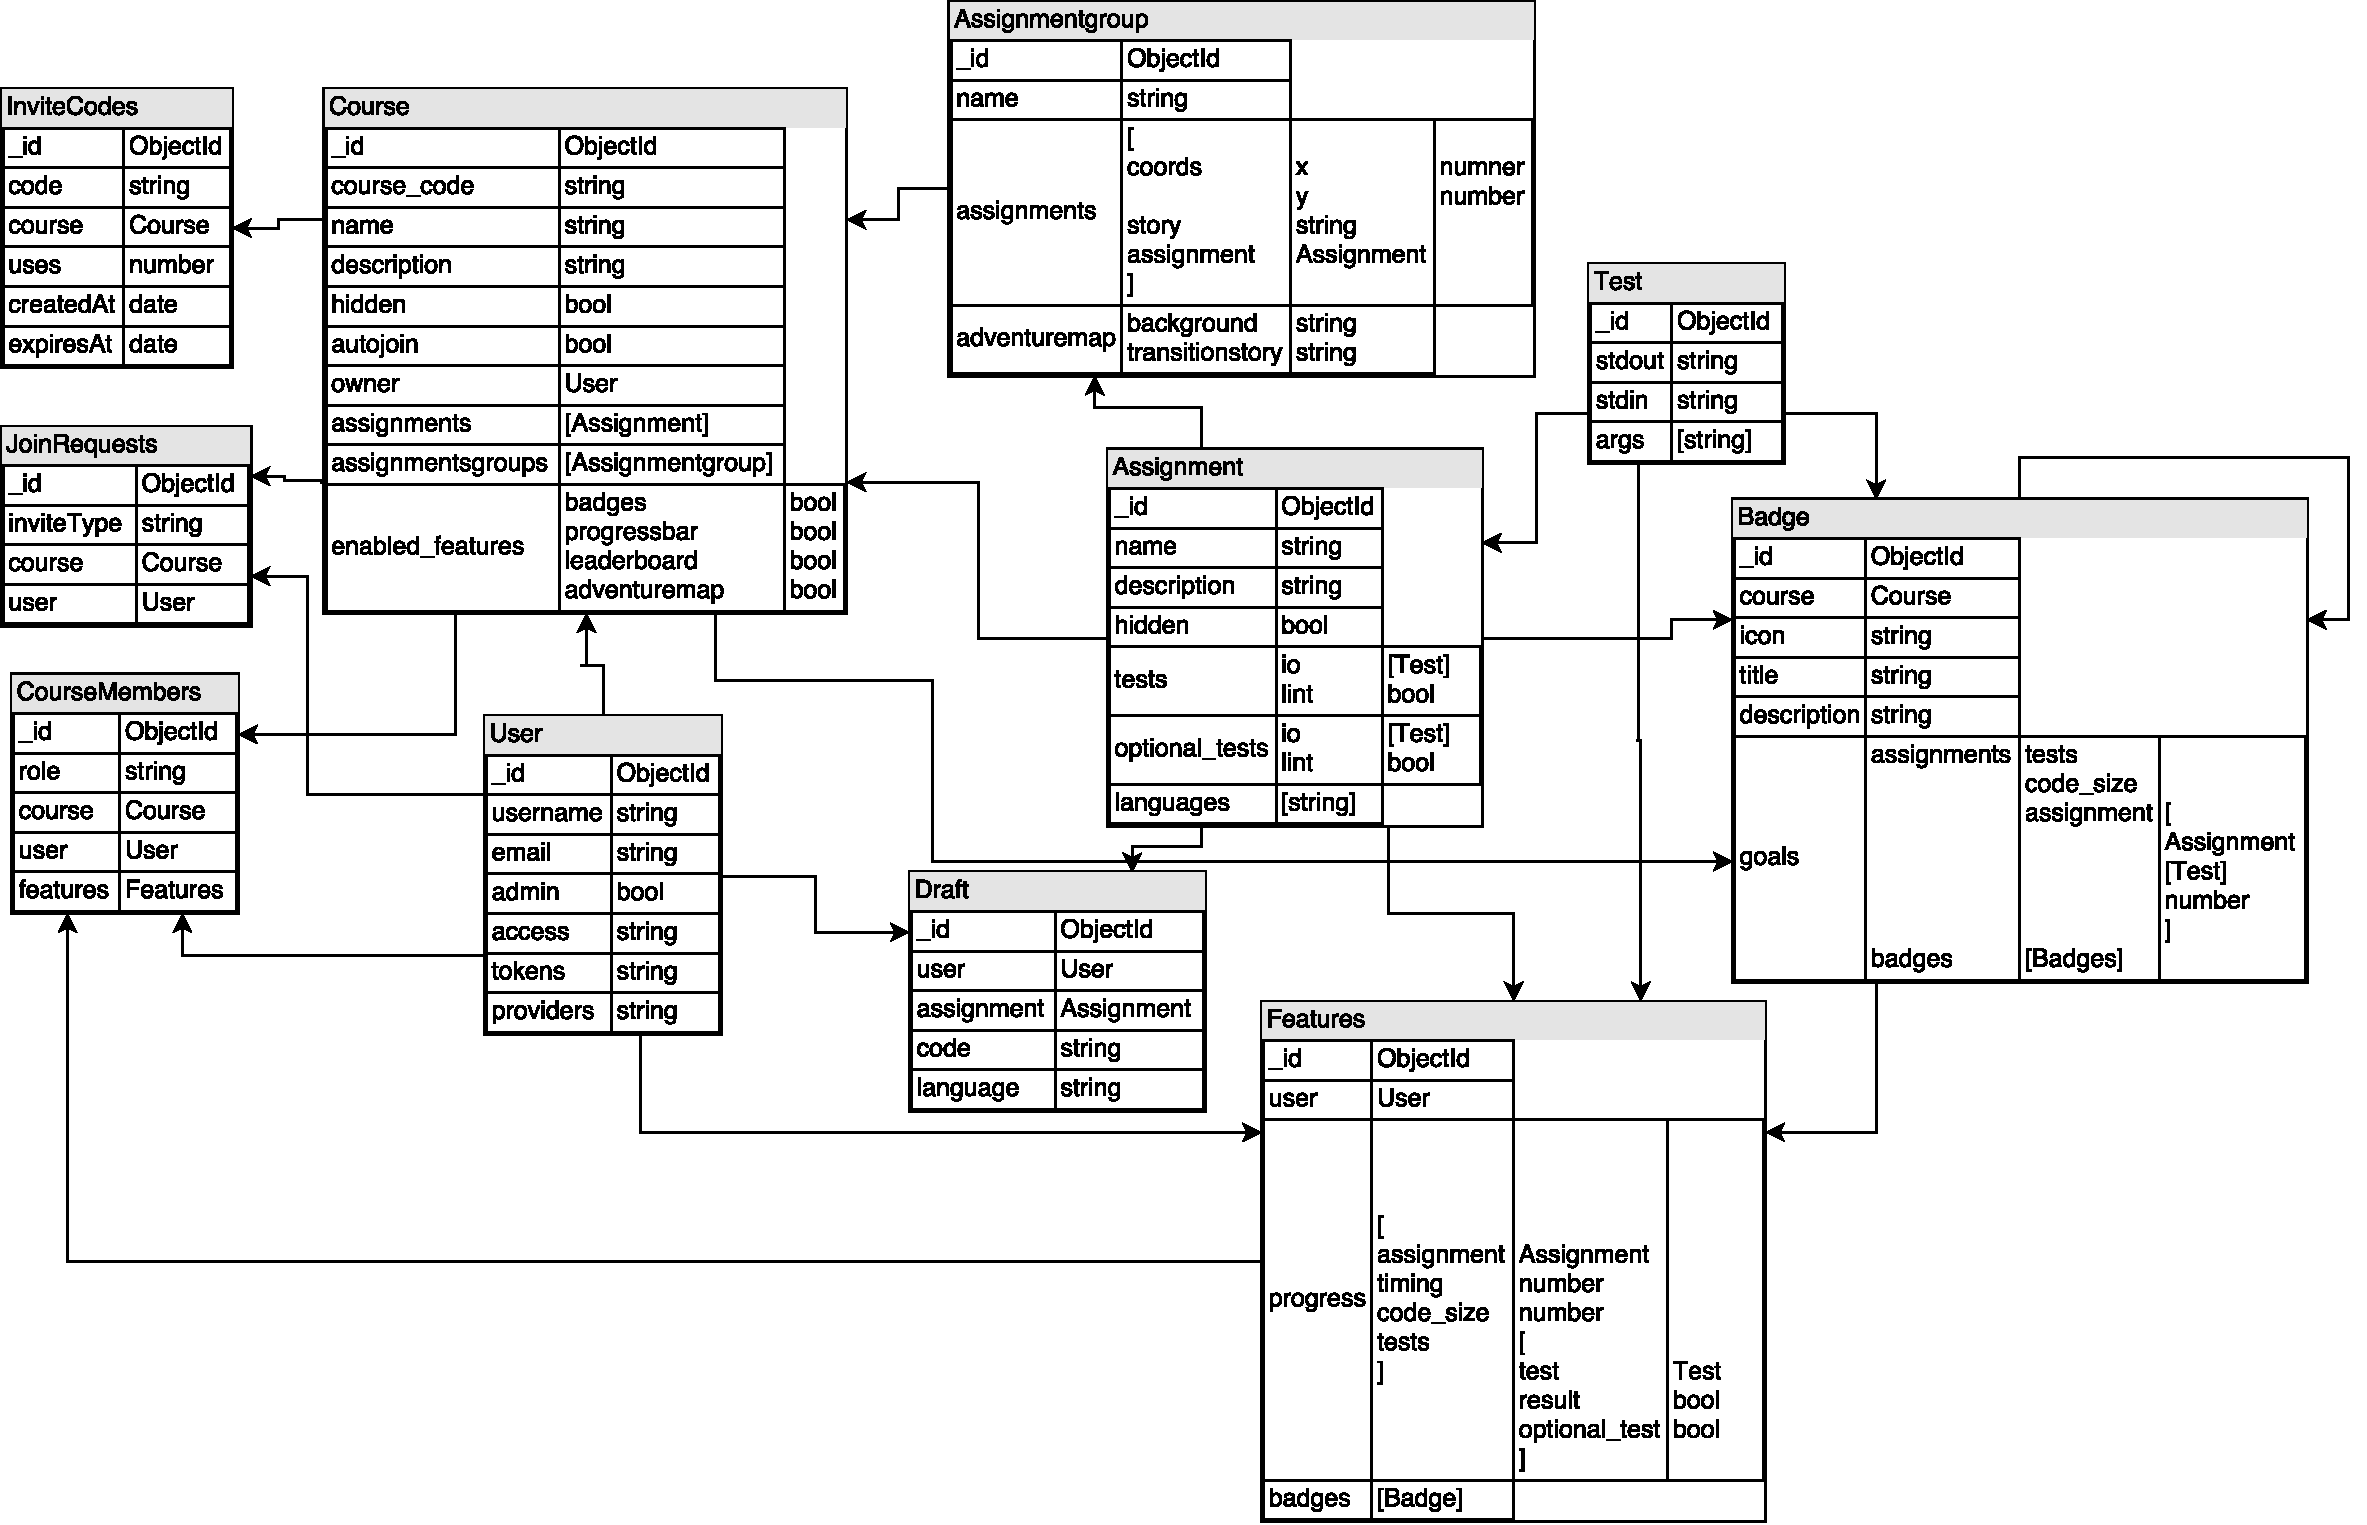
\includegraphics[width=\textwidth]{img/gpp_database-schema.pdf}
    \caption{Overview of the database schema. The arrows point from collections that are referenced to the collections that reference them.}
    \label{fig:schema}
\end{sidewaysfigure}
		
\href{https://www.mongodb.com}{MongoDB} was chosen mainly to complete the MEAN software stack (MongoDB, Express, Angular, \nodejs{}). The majority of the group members working on backend did not have prior experience working with NoSQL databases which presented a good opportunity to learn. MongoDB is a popular choice among NoSQL databases. Mongo uses a JSON-like document structure and JSON is the data format used when different parts of the project services communicate.

\href{http://www.mongoosejs.com}{Mongoose} is a package that extends MongoDB by enforcing a database structure. With Mongoose it's possible to create schemas that describe the format of the data that is to be stored in the database. Mongoose presented a problem to the project by not having consistency. If the schemas were updated there would be a mix of data, some of it stored in the previous format and some in the new. This resulted in a need to either migrate or remove the data in the database after schema updates.

While developing it also proved valuable to have a graphical representation of the data. The data was displayed using \href{https://github.com/mrvautin/adminMongo}{AdminMongo} which also enabled developers to create new entries, edit existing data and delete data. Being able to insert and edit data presented some issues throughout the project since the tool has full freedom when inserting data. No input validation or checks to the current database schemas are made. 

\subsubsection{Schema}
An overview of the database schema can be seen in figure \ref{fig:schema}. There are a number of core collections: \emph{User}, \emph{Course}, \emph{Assignment} and \emph{Test}. These core collections are essential for the base functionality of the platform. The other collections are auxiliary and were added to support additional functionality and features. For example, \emph{Assignmentgroup} makes it possible for teachers to divide course assignments into groups and is used, among other things, to support some gamification elements.

The database design started with the core collections and evolved during development to support new features that were added. Decisions needed to be made quickly to maintain the workflow, which might have resulted in some suboptimal solutions. The resulting schema was very relational, which imposed a problem as MongoDB only supports atomicity on a document level. An example of this is if a document is removed from the database, separate queries need to be made to remove any references held by other documents, which may result in inconsistencies if other queries are made at the same time. The solution to this would be to design a schema with less relations, or to use a relational database.

\subsection{API protocol}
A decision was made early in the project to adhere to a RESTful API design. Access paths to resources are built from the database schema, see figure~\ref{fig:schema}. For example: in the current database design, each assignment belongs to a course. It is therefore necessary to reference a specific course to access an assignment. Example: \texttt{GET https://.../api/courses/\allowbreak123123123/assignments/456456456/} returns assignment \texttt{456456456} which belongs to course \texttt{123123123}. Each resource name such as \texttt{courses} is in plural. A POST to \texttt{https://.../api/courses} creates a course while a GET request to the same resource returns all courses.

Data can be sent to the backend via both body and URL. Sending data via body is relevant for PUT and POST requests. The information for such requests should be sent as JSON and it should match the format specified in the API documentation. JSON is also the data-type used by the backend to return data, even when the result returned is a status code.

\subsubsection{API documentation} \label{apidocs}
Documentation for the API can at the time of writing be found at: \\ \texttt{130.240.5.119:18000/docs}. \\
In general it is found where the Backend server is deployed at: \\ \texttt{BACKEND\_IP:PORT/docs}.

% errors
\subsubsection{Error handling}
To enhance a user's experience when working with the API, it was decided that a good way to handle both user errors and server errors should be implemented.

A server error is defined as an unexpected error that could cause the server to crash and therefore become unresponsive. A server error should never prevent the server from continuing serving data from working routes. Therefore every server error is handled and returned to the user as an HTTP error, \texttt{500:\@ Internal server error}. As explained in the logging section~\ref{logging}, a server error is logged to help maintainers localize where things went wrong. This also prevents the server from crashing, but the route which threw the error will still throw the error until it's patched.

A user error is defined as any error caused by a user of the API. Trying to call a non existent route, not including input or including the wrong input are examples of user errors. If such an error is encountered it's important that the user receives feedback on what they are doing wrong. Both a fitting HTTP error code and error message should be returned. If a user has missed one required input field they should be told exactly which field is missing. All user errors are returned with an HTTP error code of 4xx.

Another type of user error occurs when the user makes a valid request which can not be handled because of restrictions implemented in the API. For example, if a user tries to modify data which they don't have access to. These errors are still considered user errors and will follow the error form of such an error.
% extensibility in features/progress/gamification

\subsection{Security}

\subsubsection{Authentication}
The API endpoint \url{/auth/login/ltu} validates a service ticket issued by CAS at \url{https://weblogon.ltu.se/cas/login} and, if successful, will issue an access token for use at the other access restricted endpoints of the API (see figure \ref{fig:auth}). The access token is a JSON Web Token with a short life span, that is tamper-proof and contains information about the user's id and access level. This approach allows the backend to remain sessionless, as the backend will validate the token at every API request. Since the access token expires quickly a refresh token is issued alongside it. The refresh token has a much longer life span and its only use is to generate new access tokens at the \url{/auth/login/accesstoken} endpoint. The refresh tokens are stored in the database, while the access tokens are not. Revoking a refresh token is done by deleting it from the database. Theft of an access token or refresh token would give the thief access until the token expires or, in the case of refresh tokens, until it is revoked. Stealing tokens is made harder with SSL encryption.

Currently logging in with CAS via \LTU\ is the only way to access the backend. This could however be extended to allow more ways of logging in by adding other authentication endpoints to the backend.

\subsubsection{HTTPS} \label{https}
Self-signed certificates have been used for the testing environment in order to establish a secure environment with HTTPS. Once a proper production environment is used, it is necessary to use a trusted certificate authority instead of self-signed certificates.

\subsubsection{Input validation}
Injection attacks are a common security problem in applications that use databases. To prevent this the API has to make sure the input has the expected form. A boolean input field must be of boolean type to be accepted. To achieve this, the module \href{https://github.com/ctavan/express-validator}{express-validator} was used. With this module it's possible to check URL, query and body input. For every invalid input field a specific error message is added to an array. When all fields have been checked, this array will be returned together with an HTTP error code 400 as feedback. This way the user can receive direct feedback without the need to consult the documentation.

% SSL (HTTPS), just mention it
\subsubsection{Access control}
The API has three different base roles, 
\begin{itemize}
\item Basic
\item Advanced
\item Admin
\end{itemize}
These are assigned according to the user's role in their school, which is found when logging in through CAS. If the user is a student, a basic role will be assigned, and if the user is a teacher, an advanced role will be assigned. Admin is never assigned automatically and has to be set manually if needed. Depending on the role, different limitations are enforced. A basic user is only allowed to create 3 courses. Admins and advanced users are allowed to create an unlimited number of courses. This is currently the only difference between a basic and an advanced user. The reason a basic user is limited in their number of courses is simply to prevent malicious behaviour. Admins have full access to every route and are not limited in any way. This is mostly affecting course routes. 

Regardless of a user's base role he has a different role in every course. Every course in turn has three user roles,
\begin{itemize}
\item Student
\item Teacher
\item Owner
\end{itemize}
A student is only allowed to do things regarding himself, such as submitting assignments or leaving the course. The teacher role maintains the course, but also controls who is allowed to join. The highest course role is the owner, which is the user that created the course. The owner can do everything a teacher is able to do, the only difference being that teachers can't remove the owner from the course. A user with the admin base role is basically able to do everything in any course.

\subsection{Quality control}
% jenkins
\subsubsection{Jenkins}
As a way to keep the project effective it was determined that it was important to implement continuous integration as a part of the project to have a modern workflow where you could push changes to git and have them automatically built on a live test server. Using continuous integration was also a good way to separate production and development builds and a way to ensure that production builds always kept a certain standard and robustness. The framework that was used for continuous integration was Jenkins which is one of the most popular frameworks.

While the idea of how continuous integration was supposed to be used in the project was quite clear, the concept wasn't put to as good use as it could have. In the first half of the project, the builds generated from Jenkins wasn't really put to use. This was mainly due to communication errors and the fact that the builds weren't needed as much. For the second part of the project the builds were used more. The way that the deployment with Jenkins was setup was to build from two branches from GIT, one from the master which was supposed to build for production and another from the backend branch which was supposed to build for development. The idea was that the development build would always contain the latest changes in backend. As the project reached its deadline it became increasingly important to also keep the backend dev builds stable because of the fact that the frontend team were depending on the backend dev build when developing.

Because of the increasing demands on having stable backend dev builds, a new requirement was setup for the continuous integration where a new development dev build was only built if it passed a set of unit-tests for the application.

% different environments
\subsubsection{Different environments}
Connected to the reasoning of building the backend in different environments/modes such as production or development, it was important to load different configurations depending on what environment the backend was supposed to run. For example, the production environment should not use the same database as the development environment. Because of this, it was important to be able to run the backend in different modes and dynamically load the correct configurations based on the mode that the backend was running in, hence a system that did this was implemented.

% logging
\subsubsection{Logging} \label{logging}
A large part of developers and support teams work is monitoring, debugging and troubleshooting. Because of this it is important to have good logging as a way to make these processes easier, faster and smoother. Having good logging gives them a good insight into what the application is doing and how it works. Because of this, it was important to have proper, useful and extensible logging available in the backend. A custom logging system promtly named logger was developed that ran with Winston and Morgan at its core. Winston is a simple and universal logging library and Morgan is a HTTP request logger middleware. Logger combined winston and morgan with the selectiveness of running the backend in different modes/environments. Depending on the mode, logger had different parts that it logged into log files.

Logger was setup to log all errors, server errors and a general logs in separate log files. When running in dev mode it was also important to log to the console, but not otherwise, hence console logging was only enabled when the backend ran in dev mode. 

Winston and Logger use levels to identify what type of information a log contains, the logging levels in logger conform closely to the severity ordering specified by RFC6424.
The severity of all levels are numerically ascending from most important to least important.

\begin{enumerate}
  \item Server Error
  \item Error
  \item Warning
  \item Info
  \item Verbose
  \item Debug
  \item Silly
\end{enumerate}

% automated testing
\subsubsection{Automated testing}
The API is a large part of the backend codebase. Automated tests of the endpoints were developed, mainly to guard against regressions. The tests mostly assert that the server doesn't return an error when given good input. In order to save time in test development, the tests are run in order, where older tests create the resources that are needed for later tests. This is not good practice in automated tests, but it would have been far more costly to make the tests independent of each other by doing setup and teardown for each endpoint test.

\subsection{Feature}

As this project had focus on adding gamification elements for programming exercises
and making programming more fun in general it was important to include
a tool that support development of future gamification modules. This tool is called
Feature and is built in such a way that it is possible to easily extend it with more
functionallity. Feature works by running all of the gamification modules and
storing the results of these modules in a Feature collection associated with
a student and a course.

In order to achieve this flexibility that future developers should be able to expand
with their gamification elements without having to learn the whole code base.
It is important to create a system that can dynamically load files and run
code on the results from Tester. This was possible by requiring all
files in a directory, \textit{modules} inside the features directory. These module-files need to follow
a given interface. They have to contain an initiation function and a function
that is called once Tester has delivered back results to Backend. 

The initiation function connects to an eventlistener that triggers once Backend
gets a result back from Tester. When this event is triggered it will call the
function that does module specfic code. It should be noted that if any of the
mandatory tests fail then Feature wont run any gamification modules. Once a module
is done calculating it can return results that will be sent back to Frontend.

Even if extensibility was of high priority when developing this tool, it was not
possible to create it truly decoupled from the rest of the code base. For example
in front of MongoDB, Mongoose is running in order to structure what is stored in
the database. This means that if a module need to store anything in the database
the database schema has to be modified in order to support the desired structure
for that module.

Such an example is the gamification element is called Progress, after
receiving the results from Tester the result is stored in the Feature collection
of that student. Resulting in data that describe the progression of that students
advancements throughout the course.

Another example is Badge, each badge has contain information that describes the
story behind it but also what goals that has to be achieved in order to earn a
certain badge. This information is stored in a seperate model in the database
schema but that is not enough. In order to be able to track badges that a student
of a course has recieved the Feature model has to be updated aswell.

This result in that Feature is somewhat decoupled from the rest of the system and
therefore one of the easiest parts to understand and extend. To create a new module
is very simple but as most of the modules need to store something that is associated
with a student in a course the database schema most likely needs to be modified aswell.
